\documentclass[12pt]{article}

\usepackage[utf8]{inputenc}
\usepackage[russian]{babel}
\usepackage{amsmath, amssymb}
\usepackage{graphicx}
\usepackage{listings}

\lstset{
	language=Python,
	keepspaces=true,
	extendedchars=\true,
	inputencoding=utf8,
	basicstyle=\tiny,
	numbers=left,
	showspaces=false,
	showstringspaces=false,
}

\def\dd#1#2{\cfrac{\partial#1}{\partial#2}}

\author{Будакян Я. С.}

\begin{document}
	\begin{titlepage}
		\begin{center}
			{\small\textsc{Московский Государственный Университет им. М.\,В. Ломоносова}}
			\vskip 1pt \hrule \vskip 3pt
			{\small\textsc{Физический факультет}}
			\vfill
			{\Large Практическое задание по ОММ}
			\break
			\break
			{\Large Задача \#2}	
		\end{center}
		
		\vfill
		
		\begin{flushright}
			{Выполнил студент 335 группы\\Будакян Я.\,С.\\
			 Преподаватель Домбровская Ж.\,О.}
		\end{flushright}
	\end{titlepage}
	
	\section{Постановка задачи}
		\bigskip\par\noindent{\bf Задача 2. }
		Используя метод переменных направлений, решите краевую задачу:
		
		\begin{equation}
			\begin{cases}
				&\dd{u}t = \Delta u \quad 0 < x < 1, \quad 0 < y < 2, \quad t > 0 \\
				&u\vert_{x=0} = u\vert_{x=1} = 0,\\
				&u\vert_{y=0} = u\vert_{y=2} = 0,\\
				&u\vert_{t=0} = \sin 2\pi x \sin \pi y
			\end{cases}
		\end{equation}
	
	\section{Метод решения}
		\subsection{Метод переменных направлений}
			Для численного решения задачи, введем двумерную пространственную и временную равномерные сетки:
			
			$$\bar{\omega}_{h_1} = \{x_i = ih_1;\ i = \overline{0,N_1};\ h_1 N_1 = 1\}$$
			$$\bar{\omega}_{h_2} = \{y_j = jh_2;\ j = \overline{0,N_2};\ h_2 N_2 = 2\}$$
			$$\bar{\omega}_\tau = \{t_k = k\tau;\ k =\overline{0,S};\ \tau S = T\}$$
			$$\bar{\omega}_{h_1 h_2 \tau} = \bar{\omega}_{h_1} \times \bar{\omega}_{h_2} \times \bar{\omega}_\tau = 
			\{ (x_i, y_j, t_k) \in \bar{D} \}$$
			$$\bar{D} = \{ 0 < x < 1;\ 0 < y < 2;\ 0 \le t \le T \}$$
			
			Введем сеточную функцию:
			
			$$\omega^k_{h_1 h_2} \overset{\mathrm{def}}{=} u(x_i, y_j, t_k)$$
			
			Запишем разностную аппроксимацию оператора Лапласа:
			
			$$L\omega \rightarrow \Lambda\omega = \Lambda_1\omega + \Lambda_2 \omega,$$
			
			где
			
			$$\Lambda_1\omega = \frac{\omega_{i-1,j} - 2\omega_{ij} + \omega_{i+1,j}}{h^2_1}$$
			
			$$\Lambda_2\omega = \frac{\omega_{i,j-1} - 2\omega_{ij} + \omega_{i,j+1}}{h^2_2}$$
			
			При решении данной задачи используется схема переменных направлений, являющаяся экономичной разностной схемой. Такая схема сочетает в себе ряд преимуществ, таких как сложность $O\left(N_1 N_2\right)$ и безусловная устойчивость.
			В этой схеме переход с одного временного слоя на другой происходит в 2 шага, привлекая промежуточный(дробный) слой. Разностная аппроксимация примет вид:
			
			$$\frac{\omega^{k+\frac{1}{2}} - \omega^k}{0.5\tau} = \Lambda_1 \omega^{k + \frac{1}{2}} + \Lambda_2 \omega^k$$
			
			$$\frac{ \omega^{k+1} - \omega^{k+\frac{1}{2}}}{0.5\tau} = \Lambda_1 \omega^{k + \frac{1}{2}} + \Lambda_2 \omega^{k+1}$$
			
			Рассмотрим переход $k \rightarrow k + \frac{1}{2}$. Используя явный вид операторов $\Lambda_1$ и $\Lambda_2$, имеем:
			
			\begin{equation}
				\begin{cases}
					\frac{\gamma_1}{2} \omega^{k+ \frac{1}{2}}_{i-1,j} - (1+ \gamma_1) \omega^{k+\frac{1}{2}}_{ij} + \frac{\gamma_1}{2} \omega^{k+\frac{1}{2}}_{i+1,j} = -\frac{\gamma_2}{2} \omega^k_{i,j-1} - (1 - \gamma_2) \omega^k_{ij} - \frac{\gamma_2}{2} \omega^k_{i,j+1} \\
					\omega^{k+\frac{1}{2}}_{0j} = \omega^{k+\frac{1}{2}}_{N_1,j} = 0 \quad j = \overline{1, N_2-1},
				\end{cases}
			\end{equation}
			
			где $\gamma_1 = \frac{\tau}{h_1^2}$, $\gamma_2 = \frac{\tau}{h_2^2}$.
			Введя обозначения:
			
			$$A^{(1)} = B^{(1)} = \frac{\gamma_1}{2}$$
			$$C^{(1)} = 1 + \gamma_1$$
			$$F^k_{ij} = \frac{\gamma_2}{2} \omega^k_{i,j-1} + (1 - \gamma_2) \omega^k_{ij} + \frac{\gamma_2}{2} \omega^k_{i,j+1},$$
		
			получим систему:
				
				\begin{equation}
					\begin{cases}
						A^{(1)} \omega^{k + \frac{1}{2}}_{i-1,j} - C^{(1)} \omega^{k+\frac{1}{2}}_{ij} + B^{(1)} \omega^{k+\frac{1}{2}}_{i+1,j} = -F^k_{ij} \\
						\omega^{k+\frac{1}{2}}_{0j} = \omega^{k+\frac{1}{2}}_{N_1,j} = 0 \quad j = \overline{1, N_2-1}
					\end{cases}
					\label{sys1}
				\end{equation}
				
			Аналогично, вводя обозначения
			
			$$A^{(2)} = B^{(2)} = \frac{\gamma_2}{2}$$
			$$C^{(2)} = 1 + \gamma_2$$
			$$F^{k+\frac{1}{2}}_{ij} = \frac{\gamma_1}{2} \omega^{k+\frac{1}{2}}_{i-1,j} + (1 - \gamma_2) \omega^{k+\frac{1}{2}}_{ij} + \frac{\gamma_2}{2} \omega^{k+\frac{1}{2}}_{i+1,j},$$
			
			получим систему для перехода $k + \frac{1}{2} \rightarrow k + 1:$
			
				\begin{equation}
					\begin{cases}
						A^{(2)} \omega^{k+1}_{i,j-1} - C^{(2)} \omega^{k+1}_{ij} + B^{(2)} \omega^{k+1}_{i,j+1} = -F^{k + \frac{1}{2}}_{ij} \\
						\omega^{k+1}_{i0} = \omega^{k+1}_{i,N_2} = 0 \quad i = \overline{1, N_1-1}
					\end{cases}
					\label{sys2}
				\end{equation}
			
			Полученные системы (\ref{sys1}), (\ref{sys2}) решаются методом прогонки.
			
		\subsection{Метод прогонки}
			Метод прогонки используется для решения систем линейный уравнений вида $Ax = F$, где $F$ - трехдиагональная матрица.
			Пусть дана система уравнений
			
			\begin{equation}
				\begin{cases}
					A_n y_{n-1} - C_n y_n + B_n y_{n+1} = -F_n, \quad n = \overline{1, N-1} \\
					A_n \neq 0, \quad B_n \neq 0, \quad n = \overline{1, N-1} \\
					y_0 = k_1 y_1 + \mu_1, \quad y_N = k_2 y_{N-1} + \mu_2
				\end{cases}
			\end{equation}
			
			Ее решение будем искать в виде:
			
			$$y_n  = \alpha_{n+1} y_{n+1} + \beta_{n+1}, \quad n = \overline{1, N-1}$$
			
			Подставляя и исключая $y_{n-1}$ и $y_n$, получаем:
			
			$$[(A_n \alpha_n - C_n)\alpha_{n+1} + B_n]y_{n+1} + [(A_n \alpha_n - C_n)\beta_{n+1} + (A_n \beta_n + F_n)]$$
			
			Получившееся уравнение будет удовлетворено вместе с граничными условиями, если
			
			$$\alpha_1 = k_1, \quad \beta_1 = \mu_1$$
			$$\alpha_{n+1} = \frac{B_n}{C_n - \alpha_n A_n}, \quad \beta_{n+1} = \frac{A_n \beta_n + F_n}{C_n - \alpha_n A_n}, \quad n = \overline{1, N-1}$$
			$$y_N = \frac{\mu_2 + \beta_N k_2}{1 - \alpha_N k_2}$$
			
			Используя эти формулы, сначала вычисляются все коэффициенты $\alpha_n, \beta_n$, а потом все неизвестные $y_{N-1}, y_{N-2}, ..., y_0$.
			
			Достаточные условия устойчивости метода прогонки:
			
			$$|C_n| \ge |A_n| + |B_n|, \quad n = \overline{1, N-1}$$
			$$|k_\alpha| \le 1, \quad \alpha = 1, 2, \quad |k_1| + |k_2| < 2$$
			
			Проверим эти условия для системы (\ref{sys1}):
			
			$$1 + \gamma_1 = |C^{(1)}| \ge |A^{(1)}| + |B^{(1)}| = \gamma_1$$
			$$k_1 = k_2 \equiv 0$$
			
			Аналогично, условия выполняются и для системы (\ref{sys2}).
			
	\section{Порядок аппроксимации}
	
	\section{Устойчивость схемы}
	
	\section{Результаты}
		Численный расчет с помощью описанного алгоритма дает следующий результаты:
		
		\begin{figure}[h!]
			\begin{minipage}[h]{0.5\linewidth}
				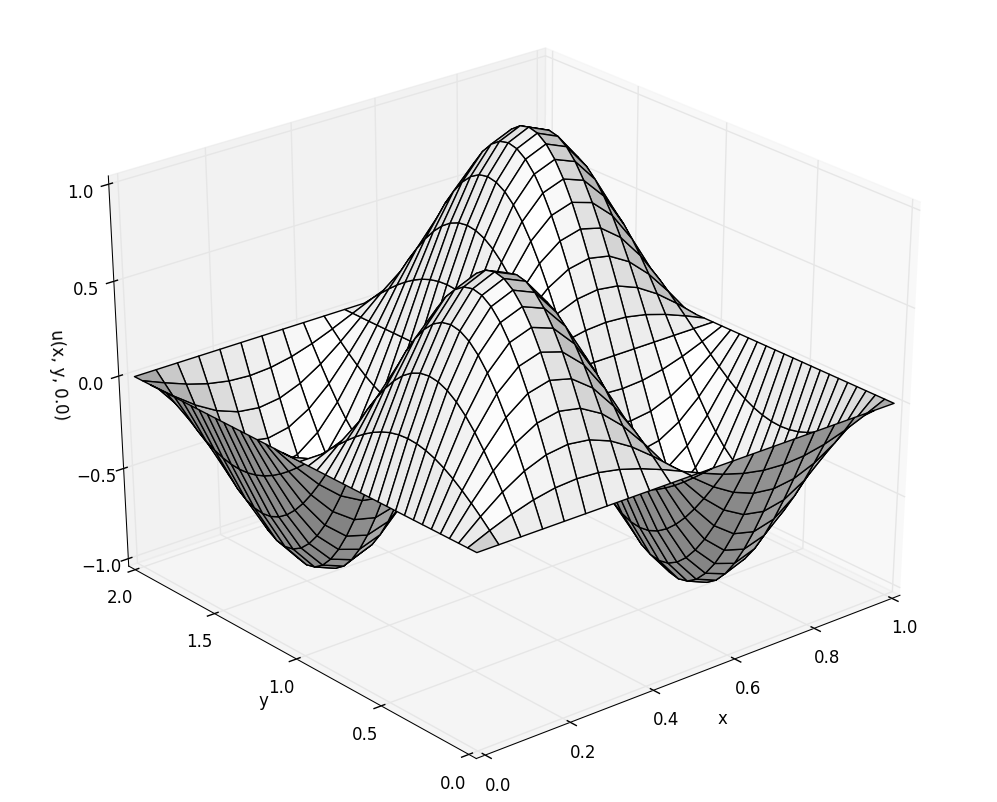
\includegraphics[width=\linewidth]{solution_t00}
				\caption{T = 0}
			\end{minipage}
			\hfill
			\begin{minipage}[h]{0.5\linewidth}
				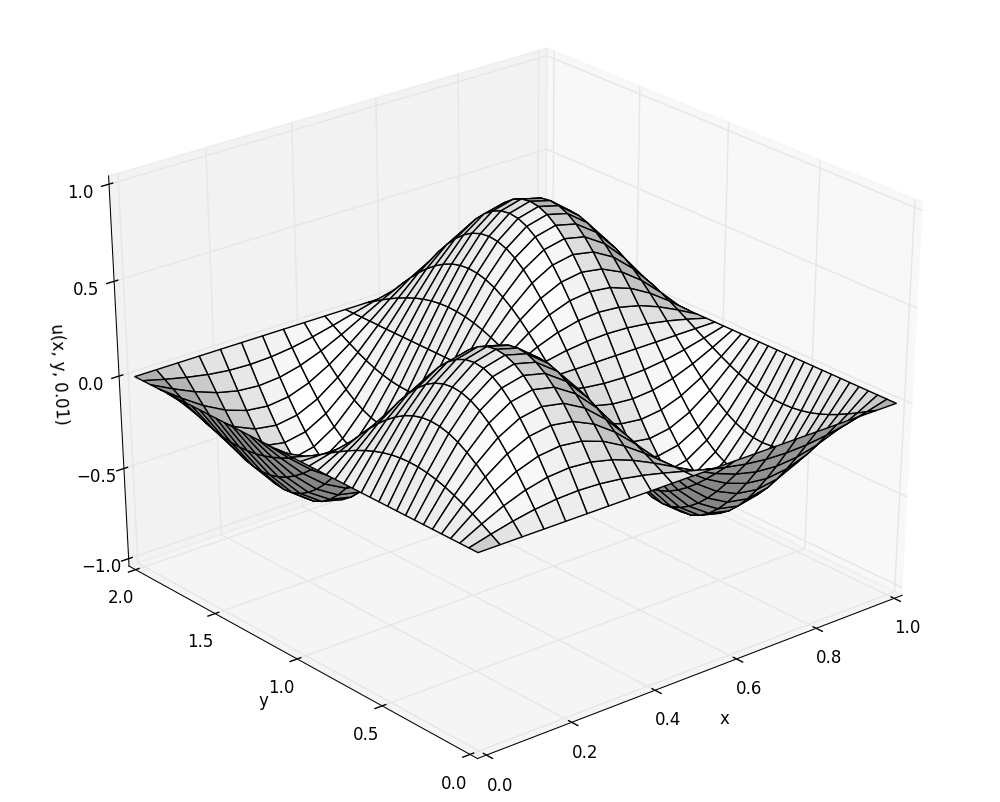
\includegraphics[width=\linewidth]{solution_t01}
				\caption{T = 0.01}
			\end{minipage}
			\vfill
			\begin{minipage}[h]{0.5\linewidth}
				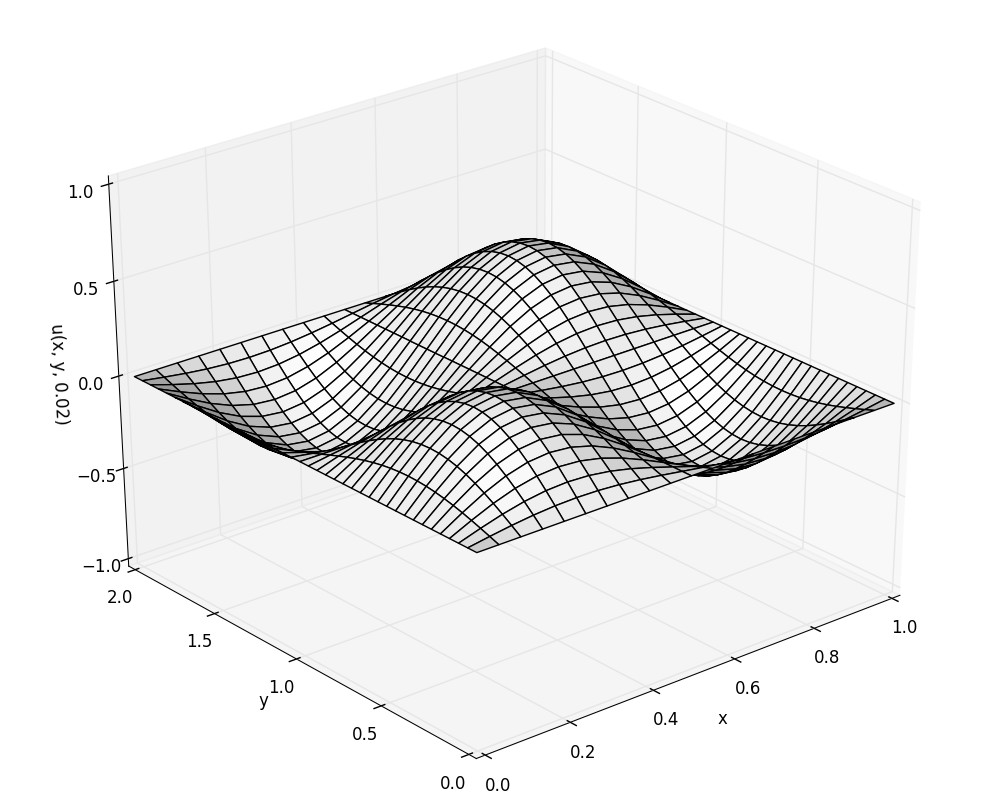
\includegraphics[width=\linewidth]{solution_t02}
				\caption{T = 0.02}
			\end{minipage}
			\hfill
			\begin{minipage}[h]{0.5\linewidth}
				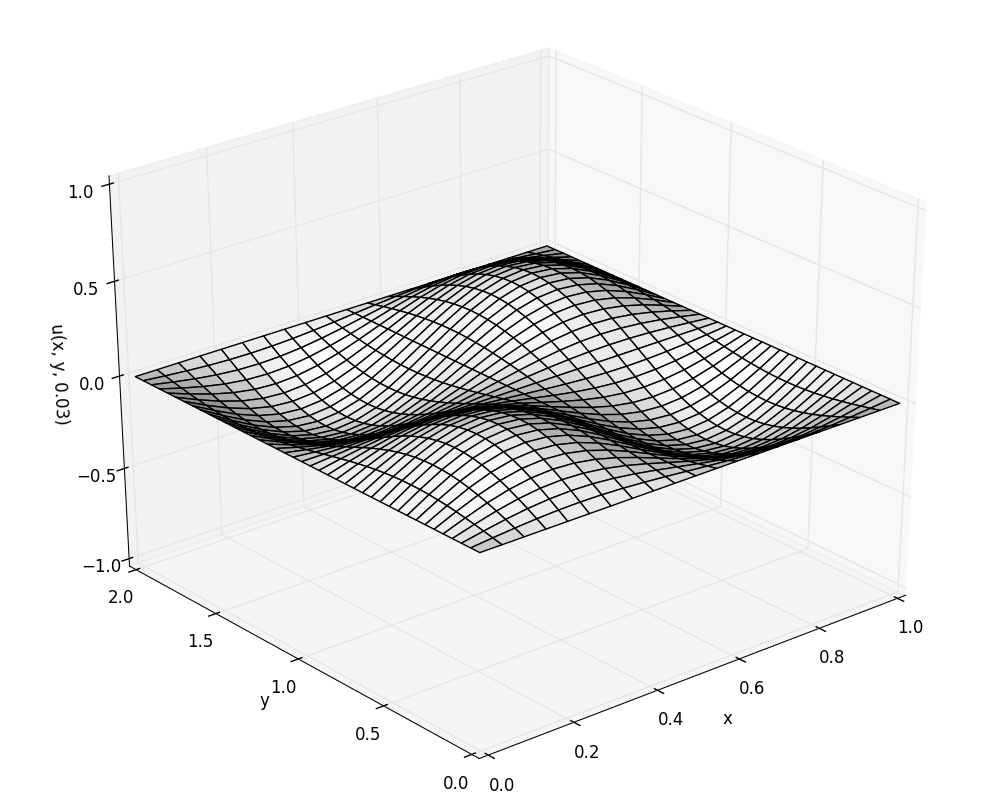
\includegraphics[width=\linewidth]{solution_t03}
				\caption{T = 0.03}
			\end{minipage}
			\vfill
			\begin{minipage}[h]{0.5\linewidth}
				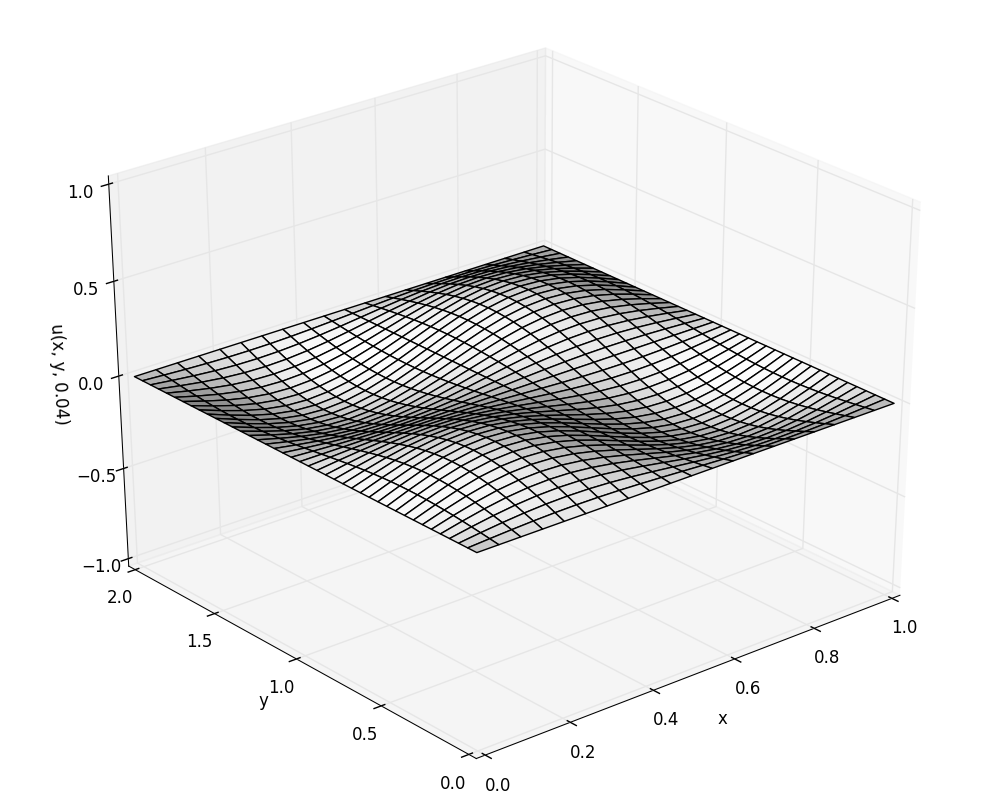
\includegraphics[width=\linewidth]{solution_t04}
				\caption{T = 0.04}
			\end{minipage}
			\hfill
			\begin{minipage}[h]{0.5\linewidth}
				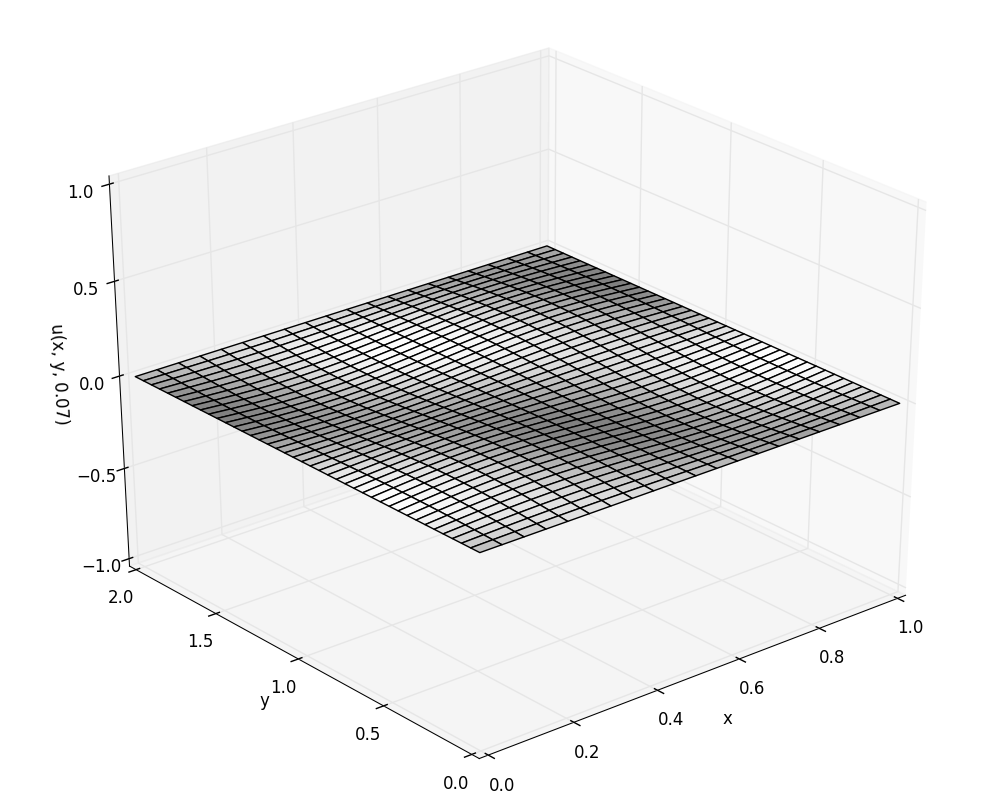
\includegraphics[width=\linewidth]{solution_t07}
				\caption{T = 0.07}
			\end{minipage}
		\end{figure}
	\newpage
	\section{Листинг программы}
	\lstinputlisting{solution.py}
	
\end{document}